\begin{problem}{Идиократия}{стандартный ввод}{стандартный вывод}{1 секунда}{256 мегабайт}

Джо Бауэрс~--- капрал, которого взяли на эксперимент по заморозке <<обычных>> людей. Со временем про него забыли. И спустя 500 лет, по стечению обстоятельств, его камера открылась. Изменилось вокруг многое: среднее значение IQ у людей упало с 110 до 20, произошла массовая деградация.

Его приводят на IQ-тест, поскольку он~--- не зарегистрированное лицо. Перед ним находится отверстие в виде \textbf{правильного выпуклого} $n$-угольника, а также имеется набор \textbf{всевозможных} фигур в форме правильных выпуклых $m$-угольников ($m \le n - 1$). 

Перед Джо поставили задачу: найти такой $k$-угольник с максимальным количеством вершин, который <<впихнется>> в данное отверстие. $k$-угольник можно \textit{впихнуть} только тогда, когда он построен на вершинах $n$-угольника (то есть все вершины $k$-угольника совпадают с некоторыми вершинами $n$-угольника), а также совпадают центры этих фигур.

\InputFile
Первая строка содержит одно целое число $t$ ($1 \le t \le 1000$)~--- количество входных тестовых наборов.

Далее в каждой строке задано число $n$ ($3 \le n \le 1000$)~--- количество вершин в отверстии.

\OutputFile
Для каждого тестового набора вывести максимальное $k$ такое, что $k$-угольник \textit{впихивается} в~$n$-угольник.

Если такой $k$-угольник отсутствует, то вывести $-1$.



\Example

\begin{example}
\exmpfile{example.01}{example.01.a}%
\end{example}

\Note
\centerline{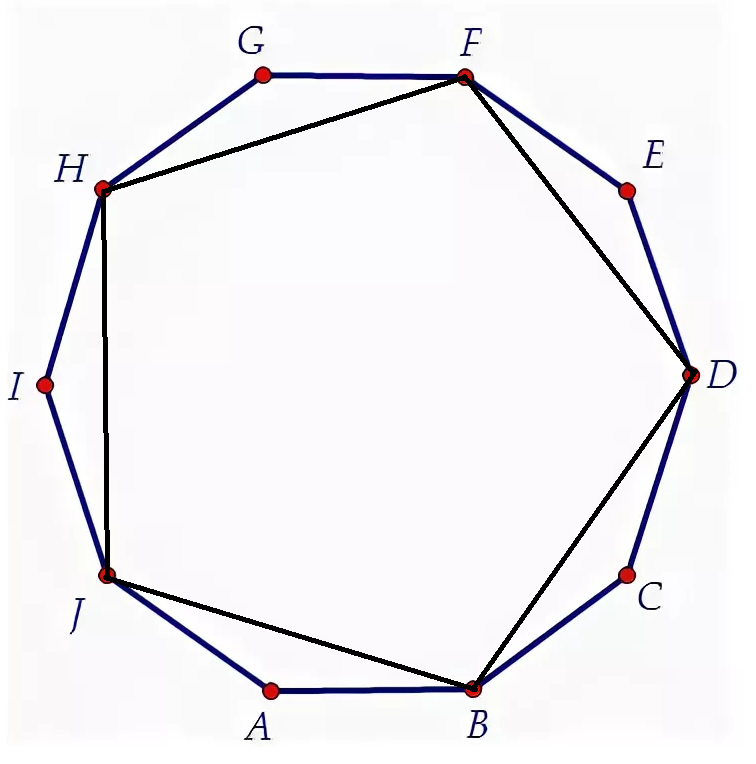
\includegraphics[scale=.35]{TaskCF.png}}

Пример построения правильного пятиугольника на правильном десятиугольнике.

Также заметим, что не существуют 1-2-угольники.

\end{problem}

